\documentclass{article}

% if you need to pass options to natbib, use, e.g.:
%     \PassOptionsToPackage{numbers, compress}{natbib}
% before loading neurips_2023

% ready for submission
\usepackage{amsmath}
\usepackage[final]{neurips_2023}
\usepackage{algorithm}
\usepackage{algpseudocode}
\usepackage{graphicx}
\usepackage{caption}

% IMPORTANT: if you are submitting attention track, please add the attention option:
% \usepackage[attention]{neurips_2023}

% to compile a preprint version, e.g., for submission to arXiv, add add the
% [preprint] option:
%     \usepackage[preprint]{neurips_2023}

% to compile a camera-ready version, add the [final] option, e.g.:
%     \usepackage[final]{neurips_2023}

% to avoid loading the natbib package, add option nonatbib:
%    \usepackage[nonatbib]{neurips_2023}

\usepackage[utf8]{inputenc} % allow utf-8 input
\usepackage[T1]{fontenc}    % use 8-bit T1 fonts
\usepackage{hyperref}       % hyperlinks
\usepackage{url}            % simple URL typesetting
\usepackage{booktabs}       % professional-quality tables
\usepackage{amsfonts}       % blackboard math symbols
\usepackage{nicefrac}       % compact symbols for 1/2, etc.
\usepackage{microtype}      % microtypography
\usepackage{xcolor}         % colors

\title{Exploring Matrix Entropy\\ Across Large Language Model Layers}

% The \author macro works with any number of authors. There are two commands
% used to separate the names and addresses of multiple authors: \And and \AND.
%
% Using \And between authors leaves it to LaTeX to determine where to break the
% lines. Using \AND forces a line break at that point. So, if LaTeX puts 3 of 4
% authors names on the first line, and the last on the second line, try using
% \AND instead of \And before the third author name.

\author{%
  Yichong Liang\\
  Department of Computer Science\\
  Colorado School of Mines\\
  Golden, CO 80401 \\
  \texttt{yichongliang@mines.edu} \\
  % examples of more authors
  % \And
  % Coauthor \\
  % Affiliation \\
  % Address \\
  % \texttt{email} \\
  % \AND
  % Coauthor \\
  % Affiliation \\
  % Address \\
  % \texttt{email} \\
  % \And
  % Coauthor \\
  % Affiliation \\
  % Address \\
  % \texttt{email} \\
  % \And
  % Coauthor \\
  % Affiliation \\
  % Address \\
  % \texttt{email} \\
}

\begin{document}

\maketitle

\begin{abstract}
This study explores the matrix entropy across layers in GPT-2 models 85M, 302M, and 708M parameters, and Tiny Story models with 3M and 28M parameters, to understand how their process and interpret narrative content. By analyzing the matrix entropy behavior of models we investigate how different narratives—specifically child stories and world stories classified into good, bad, utopian, and dystopian themes—affect the information processing capabilities of these models. The entropy analysis reveals that models are sensitive to narrative quality, with well-crafted stories eliciting higher entropy values, indicating more complex information processing. Larger models demonstrate a smoother entropy curve across layers but also exhibit greater variability in layer responses, suggesting nuanced processing that could be both an advantage and a challenge. This study not only sheds light on the interpretability of neural network models in handling narrative complexities but also underscores the importance of model architecture in achieving consistent processing across layers. Future work will expand this analysis to a wider range of datasets to further validate and refine our understanding of how structural differences in models influence their interpretability and functionality. My code is available at \url{https://github.com/YichongLiang/Exploring-Matrix-Entropy-Across-LLM-Layers.git}
\end{abstract}

\section{Introduction}


\subsection{Overview}

In the rapidly evolving field of natural language processing, large language models (LLMs) have become a cornerstone, offering unprecedented capabilities in understanding and generating human-like text. However, as these models grow in complexity and scale, evaluating their performance and the nuances of their internal mechanisms becomes a daunting challenge. Traditional evaluation metrics often fall short in providing a holistic view of a model's linguistic and cognitive abilities. Inspired by Wei \cite{wei2024}, "Large Language Model Evaluation via Matrix Entropy," this project seeks to pioneer a novel approach to probing the inner workings of LLMs by examining the matrix entropy of their embedding layers.

Matrix entropy, a concept derived from information theory, quantifies the amount of information or uncertainty in a system. By applying this metric to the embedding layers of LLMs, this project aims to unveil new insights into how information is processed and represented across different layers of the models. Wei's research revealed that matrix entropy correlates with the scale of models, providing an intrinsic measure of a model's ability to compress and structure information efficiently. This scaling law behavior of matrix entropy is particularly intriguing because it persists even when traditional metrics like loss and perplexity have plateaued, suggesting that matrix entropy captures aspects of model behavior that are invisible to conventional evaluations.

The innovation of this project lies in its unique approach: no previous studies have applied matrix entropy in this context, making it a pioneering effort in the field. This method could potentially offer a more granular and informative perspective on the 'thought process' of LLMs, leading to better understanding and improvements in model architectures. Furthermore, the findings could have significant implications for the design and training of future LLMs, enhancing their efficiency and efficacy in handling complex linguistic tasks.

This project not only aligns with the ongoing discourse on LLM evaluation but also contributes a novel methodology that could set a precedent for future explorations in the field. By blending concepts from information theory with cutting-edge machine learning, we aim to bridge the gap between theoretical metrics and practical model evaluation, offering a fresh lens through which to assess the capabilities of large language models.

\subsection{Motivation}

This project is significant because it pioneers the application of matrix entropy across the layers of LLMs, an approach not previously explored. By systematically measuring matrix entropy from the embedding to the output layers, we anticipate uncovering new insights into how LLMs process and transform information layer-by-layer. This could fundamentally enhance our understanding of how different layers contribute to the overall functionality of the models, potentially leading to more targeted and efficient model architectures.

Moreover, the application of matrix entropy as a metric allows for a more nuanced evaluation of model performance, beyond what is achievable with traditional metrics. By correlating changes in matrix entropy with modifications to model architecture or training procedures, we can gain a deeper understanding of how specific changes affect the model's internal information processing strategies. This could be crucial for developing more robust, efficient, and interpretable LLMs, thereby pushing the boundaries of what these models can achieve. In essence, this project not only builds upon the intriguing findings of Wei et al. but also expands the utility of matrix entropy from a theoretical curiosity into a practical tool for model analysis and improvement. This could set a new standard for evaluating and understanding the increasingly complex LLMs that are at the forefront of advancements in artificial intelligence.

\section{Related Work}
\label{gen_inst}

As the landscape of large language models (LLMs) continues to expand, the challenge of effectively evaluating their capabilities has become increasingly complex. Traditionally, metrics such as perplexity and cross-entropy loss have been the cornerstones of this evaluation, primarily due to their ability to measure a model's predictive accuracy. In their seminal work, Xu et al \cite{xu2024}. in "Understanding the Role of Cross-Entropy Loss in Fairly Evaluating Large Language Model-based Recommendation," highlight the importance of cross-entropy loss within recommendation systems. They convincingly demonstrate that while this metric is effective in assessing predictive performance, it falls short in probing the deeper linguistic and semantic processing capabilities of LLMs. This revelation has prompted me to consider the limitations of current evaluation methodologies, where the nuanced understanding of language by these models remains underexplored.

In contrast, Wei et al. in their pioneering study "Large Language Model Evaluation via Matrix Entropy," propose matrix entropy as a novel metric to assess the intrinsic qualities of LLMs. This metric evaluates the efficiency of data compression within models, revealing how information is structured and reduced internally. By focusing on the geometric and information-theoretical properties of model functionality, matrix entropy offers a profound insight into the internal mechanics of LLMs beyond mere output accuracy.

However, Wei et al.'s application of matrix entropy is confined mainly to a single embedding layer, which may not capture the full complexity of LLM architectures. Recognizing this gap, we am motivated to extend their methodology across multiple layers of LLMs. By applying matrix entropy more broadly, we aim to uncover detailed insights into how information is processed and transformed throughout the entire network, enhancing our understanding of these sophisticated systems.

Furthermore, the field is recognizing the need for more diverse evaluation metrics that address specific aspects of LLM applications, such as ethical considerations, fairness, and societal impacts. These considerations underscore the importance of developing holistic evaluation frameworks that not only assess technical performance but also consider the broader implications of deploying these models in real-world scenarios.

In summary, our work is part of an evolving dialogue in the field that seeks to bridge the gap between traditional metrics and more nuanced, comprehensive evaluation methods. By enhancing the methodology to include a multi-layered analysis through matrix entropy, we contributed to setting new standards for understanding and improving the capabilities of large language models.



\section{Methodology}

\subsection{Hypothesis}
The core hypothesis of my project is that matrix entropy, when measured across different layers of large language models (LLMs), can reveal deeper insights into the internal dynamics and information processing capabilities of these models. By comparing matrix entropy across various models and sizes—specifically, Tiny story, GPT-2 small, medium, and large. This aim to uncover how these models manage and transform linguistic information at different layers. Using different kinds of sets of data to prompt the model we can also notice different perspective of the internal of the model. Since we will able to see how different data affect the matrix entropy changes across the model's layers. So that the results might help us know the internal of LLMs better.

\subsection{Experiments}
To test this hypothesis, we have conducted a series of experiments involving several LLMs, using a range of prompts that vary in complexity and thematic content. Calculate the matrix entropy across the model's layers. After that calculate mean value and standard deviation to shows the statistic information. The details of experimental setup can be found below. 

\subsubsection{Model Setup} The experiments had configured multiple instances of LLMs, specifically Tiny story, and GPT-2 in its small, medium, and large configurations. Each model will be evaluated using the same set of prompts to ensure consistency in the comparative analysis.
Matrix Entropy Calculation: For each model response, we have calculated the matrix entropy across all layers of the model. The matrix entropy is calculated using the following formulas from Wei's et al paper:

Given a set of embeddings $S = \{\mathbf{z}_i \in \mathbb{R}^{d \times 1}\}_{i=1}^N$, we define the mean vector $\bar{\mathbf{z}} = \frac{1}{N} \sum_{i=1}^N \mathbf{z}_i$ and $\tilde{\mathbf{z}}_i = \frac{\mathbf{z}_i - \bar{\mathbf{z}}}{\|\mathbf{z}_i - \bar{\mathbf{z}}\|_2}$. Then the covariance matrix is constructed as
\[
\Sigma_S = \frac{1}{N} \sum_{i=1}^N \tilde{\mathbf{z}}_i (\tilde{\mathbf{z}}_i)^T.
\]
It can be easily seen that $\operatorname{tr}(\Sigma_S) = 1$.

Let \( K \in \mathbb{R}^{d \times d} \) be a positive semi-definite matrix satisfying \( \text{tr}(K) = 1 \). The matrix entropy is defined as:
\[
H(K) = -\text{tr}(K \log K).
\]
It is a well-established principle that, given the eigenvalues (spectrum) of \( K \) denoted as \( \lambda_1 \geq \ldots \geq \lambda_d \), the matrix entropy can be represented in terms of the Shannon entropy \cite{Shannon1948} over the spectrum as follows:
\[
H(K) = -\sum_{i=1}^d \lambda_i \log \lambda_i.
\]

where K is the covariance matrix of the embeddings produced by each layer, and 
tr denotes the trace of the matrix.

Assemble the formulas and we can get matrix entropy calculation algorithm from Wei's et al.

A sentence representations \( S = \{\mathbf{z}_i\}_{i=1}^N \), where \( \mathbf{z}_i \in \mathbb{R}^{d \times 1} \), \( d \) is hidden dimension of representation and \( N \) is the length.

\begin{algorithm}[H]
\caption{Matrix Entropy Calculation Algorithm}
\label{alg:matrix_entropy}
\begin{algorithmic}[1]
\State Calculate the mean vector $\bar{\mathbf{z}} = \frac{1}{N} \sum_{i=1}^N \mathbf{z}_i$
\State Normalize: $\tilde{\mathbf{z}}_i = \frac{\mathbf{z}_i - \bar{\mathbf{z}}}{\|\mathbf{z}_i - \bar{\mathbf{z}}\|_2}$
\State Construct the covariance matrix: $\Sigma_S = \frac{1}{N} \sum_{i=1}^N \tilde{\mathbf{z}}_i (\tilde{\mathbf{z}}_i)^T$
\State Compute matrix entropy: $H(\Sigma_S) = -\frac{\text{tr}(\Sigma_S \log \Sigma_S)}{\log d}$
\State Return the matrix entropy $H(\Sigma_S)$
\end{algorithmic}
\end{algorithm}


\subsubsection{Software Tools} The experiments were conducted using the Python programming language. Leveraging libraries such as transformer lens \cite{nanda2022} for it's hooked open source model, and transformer lens has much wider varieties options on model manipulation compare to similar libraries. The experiments has also leveraged PyTorch \cite{paszke2019} on mathematical operations. The covariance matrices and matrix entropy calculations that performed have also developed and calculated using PyTorch.

\subsubsection{Datasets} 
\textbf{Child Stories:} This dataset comprises a collection of narratives designed to represent typical children's literature, including elements such as simplicity, morality, and a clear narrative arc. The dataset includes both "good" stories, which are well-structured and rich in content, and "bad" stories, which lack narrative depth and complexity. Additionally, each story is presented in both its original and condensed forms, allowing for an analysis of how narrative detail impacts model performance.

\textbf{World Stories:} Composed of utopian and dystopian narratives, this dataset offers a broader spectrum of thematic complexity and moral ambiguity compared to the child stories. Utopian stories in this dataset depict idealistic societies and positive outcomes, intended to challenge the model's ability to process optimistic and complex societal constructs. Conversely, dystopian stories provide narratives filled with conflict, challenges, and darker themes, testing the model's capacity to handle narratives that incorporate intricate plots and deep philosophical questions.

\subsection{Data Analysis} The resulting matrix entropy values will be analyzed to determine patterns related to model size, complexity of the prompts, meaning of the prompts and depth of the layer within the network. This analysis will help in understanding how different architectures handle information compression and transformation internally.




\section{Results}
\label{others}

\subsection{Good \& Bad Child Stories Results}

In this section, we present the analysis of matrix entropy across various layers of the models at different scales. Each model was systematically prompted with a set of 10 good and 10 bad child stories, alongside their condensed versions, totaling 40 prompts per model. All stories were generated by GPT-4. The purpose of choosing child stories is because that Tiny story model is trained by tiny child story it will be interesting to see how the results changes between story specific model and non-specific models. This approach allowed us to capture a broad spectrum of the model's response characteristics to different narrative qualities and lengths. The plots displayed here represent the mean matrix entropy values and their standard deviations, calculated from these responses. This method provides a comprehensive view of how each model processes and encodes the information presented in the stories, highlighting differences in complexity and processing depth depending on the story's quality and condensation.


\subsubsection{Tiny Story Model}
The graphs presented illustrate the mean matrix entropy across different layers of two language models, one with 3M parameters and another with 28M parameters, highlighting their responses to good (Blue line), bad (Red line) long and condensed version of child stories.

In the Figure 1 featuring the Tiny Stories model with 3 million parameters, we observe the matrix entropy for both good and bad child stories across the layers. The higher blue line, representing good child stories in their longer version, suggests that the model processes these stories with greater complexity or variability compared to the red line, which represents bad child stories. This trend indicates that the model potentially captures more intricate patterns in well-constructed narratives. Additionally, for both good and bad stories, the condensed versions (lower blue and red lines) exhibit lower entropy values, suggesting less complexity or variability in the embeddings of these condensed texts compared to their extended counterparts.

Moving to the Figure 2, which showcases the behavior of a larger model with 28 million parameters, a similar trend is evident where good stories (blue lines) typically show higher entropy than bad stories (red lines). However, this model demonstrates a more stable entropy profile across its layers compared to the 3M model, indicating a uniform processing capacity that might reflect better generalization across different types of content. It's notable that the difference in entropy between good and bad stories is less pronounced in this model, which could suggest that it handles narrative quality more consistently.

Overall, these results underscore a clear pattern where longer and qualitatively better stories tend to yield higher entropy across both models. This pattern supports the notion that more text—and presumably more complex text—provides a richer context for the models to process, which is reflected in higher entropy values. Additionally, the relatively stable entropy values across the layers in the larger model might indicate its ability to maintain consistent processing abilities regardless of the narrative quality, a feature that is less prominent in the smaller model. These insights are crucial for understanding how story quality and length influence the behavior of language models and could guide further research into optimizing model architectures for varied narrative complexities.

\begin{figure}[H]
    \centering
    \begin{minipage}{0.5\linewidth}
        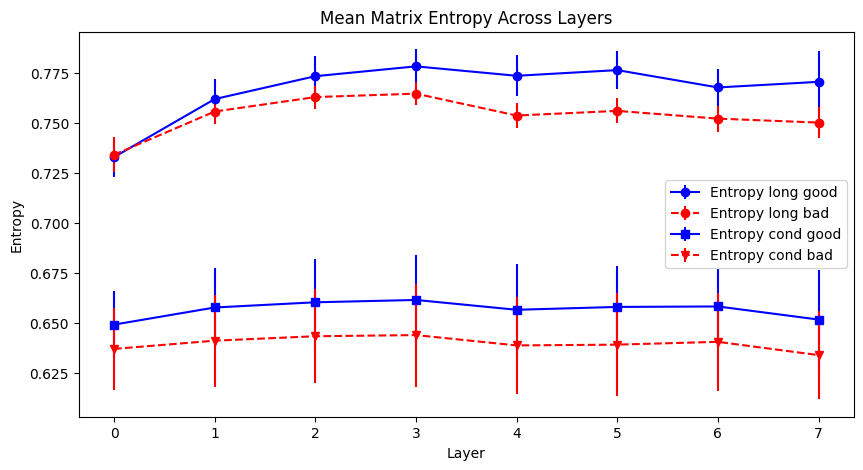
\includegraphics[width=\linewidth]{Tiny_Child_Stories.png}
        \caption{Tiny Story Model (3M) Child Stories}
        \label{fig:Tiny_child}
    \end{minipage}\hfill
    \begin{minipage}{0.5\linewidth}
        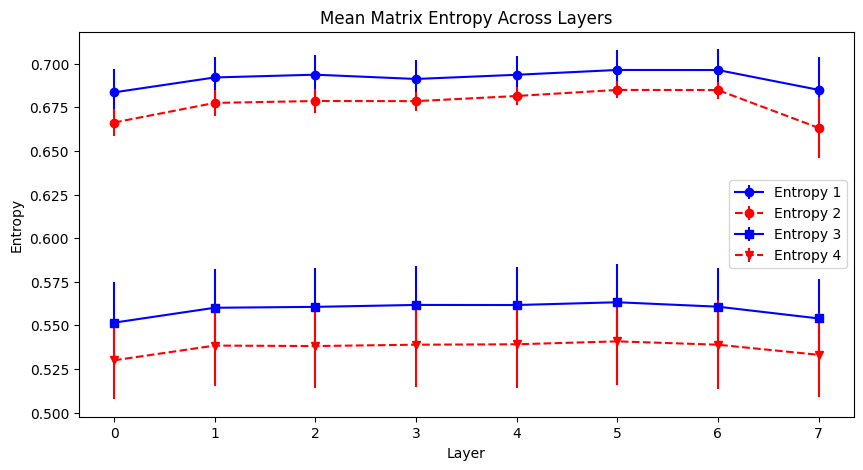
\includegraphics[width=\linewidth]{Tiny_l_Child_Stories.png}
        \caption{Tiny Story Model (28M) Child Stories}
        \label{fig:Tiny_l_child}
    \end{minipage}\hfill
\end{figure}


\subsubsection{GPT-2}

The plots depicted illustrate the mean matrix entropy across layers for GPT-2 models of different scales—small (85M parameters), medium (302M parameters), and large (708M parameters)—analyzing their responses to child stories, both good (Blue line) and bad (Red line), along with their condensed and longer versions.

In the case of GPT-2 Small, illustrated in Figure 3, the entropy values across layers show a distinct trend, with good stories, both long and condensed, typically registering higher entropy than their bad counterparts. This indicates a more complex or varied information processing pattern for good stories. Despite the smaller scale of this model, the pattern of entropy changes distinctly between layers, particularly in the transition from initial to middle layers where entropy spikes before gradually stabilizing.

Moving to the GPT-2 Medium, shown in Figure 4, which possesses a higher parameter count and more layers, the pattern is notably smoother compared to the small model. Good stories again tend to exhibit higher entropy across the layers. The progression of entropy values is more consistent, with less dramatic changes between consecutive layers, suggesting a more uniform processing capability that might be attributed to the increased complexity and depth of the model.

Lastly, the GPT-2 Large model displayed in Figure 5, the largest among the three, maintains a similar pattern where good stories outpace bad stories in terms of entropy. This model shows a very consistent entropy profile across its extensive layer structure, indicating robustness in processing and perhaps a better generalization ability across different story qualities. The layers manage entropy with slight fluctuations but maintain a clear distinction between the quality of stories.

Across all three models, there is a noticeable consistency in how good stories generally result in higher entropy, signifying more complex processing patterns. The number of parameters and layers in each model influences how smooth the entropy curve appears, with larger models showing less variability between layers, reflecting their capability to process information more uniformly. This uniformity and smoothness in the entropy curve enhance as the model size increases, illustrating a potential increase in the ability to handle diverse linguistic features and story complexities more effectively.



\begin{figure} [H]
    \centering
    \begin{minipage}{0.5\linewidth}
        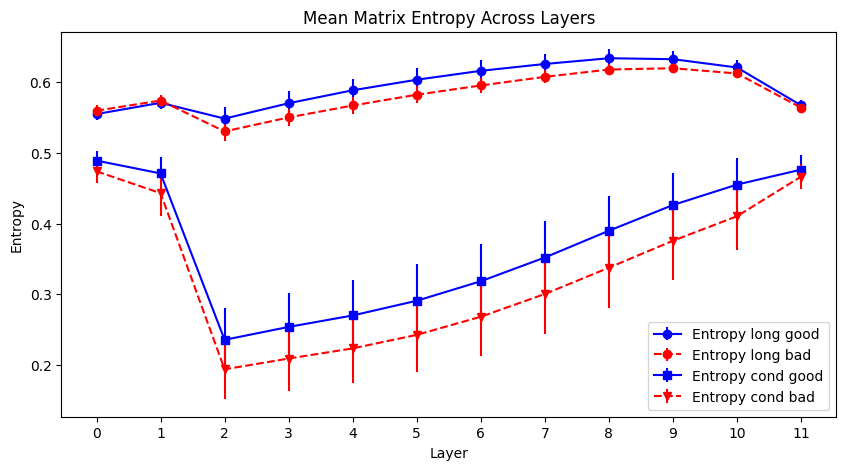
\includegraphics[width=\linewidth]{Small_Child_Stories.png}
        \caption{GPT-2 Small (85M) Child Stories}
        \label{fig:small_child_stories}
    \end{minipage}\hfill
    \begin{minipage}{0.5\linewidth}
        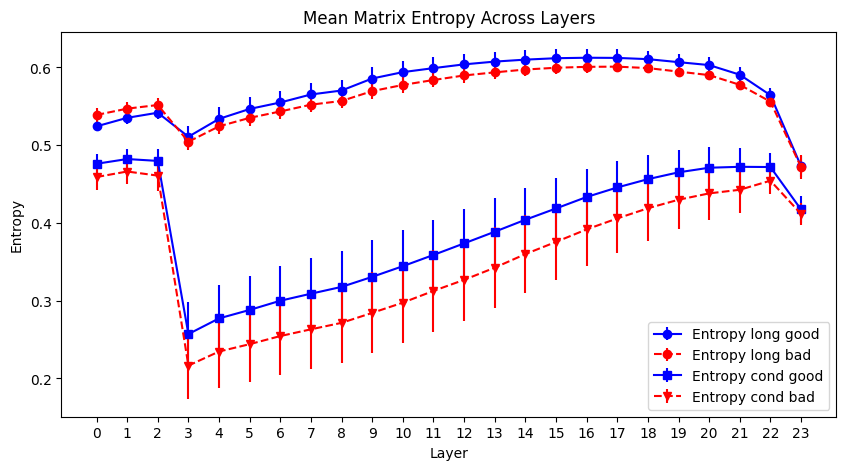
\includegraphics[width=\linewidth]{Medium_Child_Stories.png}
        \caption{GPT-2 Medium (302M) Child Stories}
        \label{fig:medium_child_stories}
    \end{minipage}\hfill
\end{figure}



\begin{figure} [H]
\centering
    \begin{minipage}{0.5\linewidth}
        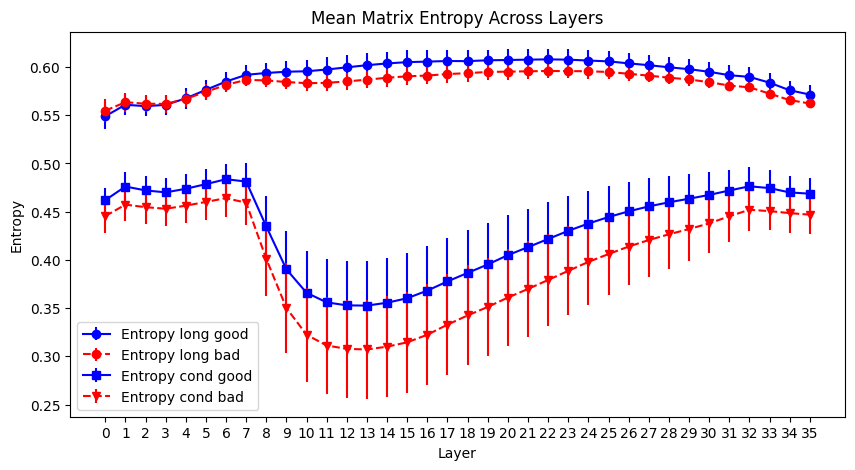
\includegraphics[width=\linewidth]{Large_Child_Stories.png}
        \caption{GPT-2 Large (708M) Child Stories}
        \label{fig:large_child_stories}
    \end{minipage}
\end{figure}





\subsection{Utopian \& Dystopian World Stories Results}

Similarly to the last subsection this subsection delves into the matrix entropy analysis across different layers of the models, each scaled variably from small to large. To explore how these models handle thematic complexity and narrative structures, we prompted them with a series of 10 Utopian and 10 Dystopian stories all generated by GPT-4. The purpose of choosing this kind of stories is because this is kind of like adult version of good and bad stories. This making a total of 20 unique narrative prompts for each model. This analysis focuses on how well different models process and interpret the distinct thematic elements and moral complexities embedded within these genres. The ensuing figures illustrate the mean matrix entropy values and their standard deviations, derived from the responses to these stories. By examining these metrics, we gain insights into the model's ability to encode and differentiate between the underlying themes of utopia and dystopia, reflecting their capacity for thematic sensitivity and narrative comprehension.

\subsubsection{Tiny Story Model}

The analysis depicted in Figures 6 and 7 examines the mean matrix entropy across different layers of two variations of the Tiny Story model, one with 3M parameters and the other with 28M parameters. These figures provide insights into how each model processes utopian (blue line) versus dystopian (red line) narratives.

In Figure 6, representing the Tiny Story Model with 3M parameters, the matrix entropy shows distinct patterns for utopian and dystopian stories. The entropy for utopian stories exhibits a relatively stable trend with a peak around layer 4, suggesting that this layer may be pivotal in processing complex themes associated with idealistic scenarios. Conversely, the entropy for dystopian stories is more variable across layers, peaking earlier around layer 3 and then showing a downward trend. This variability could imply that the model processes dystopian themes with differing levels of complexity and uncertainty, possibly due to the inherently conflict-driven and varied nature of dystopian narratives.

Figure 7 shows a similar analysis for the Tiny Story Model with 28M parameters. Here, the model's response to utopian stories is noticeably more stable across all layers compared to its handling of dystopian stories, which exhibit greater fluctuation in entropy. This model, despite having more parameters, still demonstrates a clear distinction in how it processes the two different narrative types. The utopian narratives maintain higher entropy levels throughout, suggesting a consistent handling of these themes, while the dystopian narratives show a more pronounced decrease in entropy from the middle layers onwards, indicating a potential reduction in narrative complexity or a convergence towards certain predictable patterns.

Across both models, it is evident that utopian stories generally maintain higher and more stable entropy levels compared to dystopian stories. This pattern could reflect the model's efficiency and consistency in encoding utopian narratives, which may be more straightforward or less varied than dystopian ones. On the other hand, the fluctuating entropy in dystopian stories across both models suggests these narratives challenge the models differently, possibly due to their complex, variable, and often darker themes that require nuanced understanding and processing.


\begin{figure}[H]
    \centering
    \begin{minipage}{0.5\linewidth}
        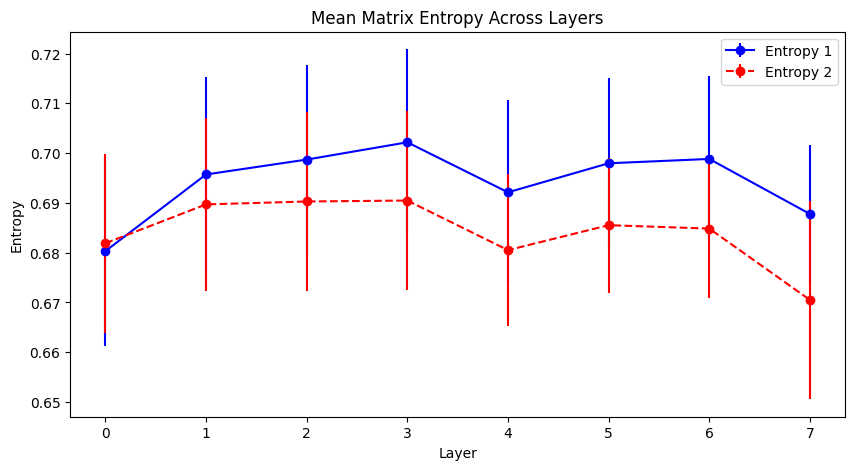
\includegraphics[width=\linewidth]{Tiny_Word_Stories.png}
        \caption{Tiny Story Model (3M) World Stories}
        \label{fig:Tiny_world}
    \end{minipage}\hfill
    \begin{minipage}{0.5\linewidth}
        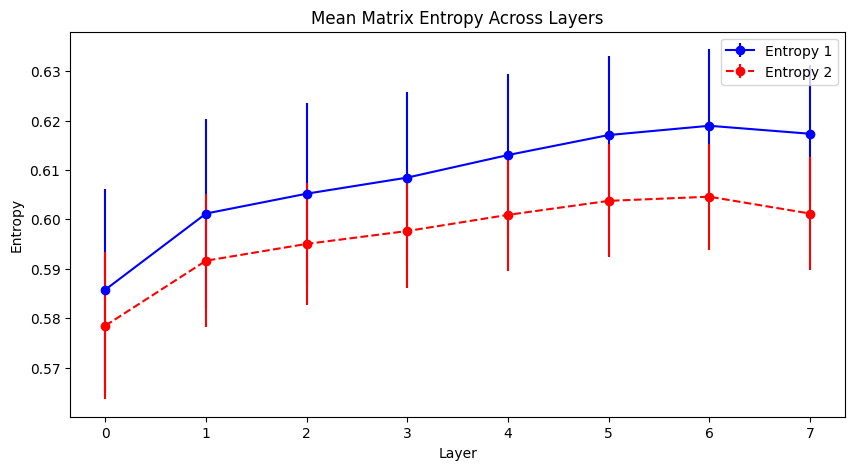
\includegraphics[width=\linewidth]{Tiny_l_World_Stories.png}
        \caption{Tiny Story Model (28M) World Stories}
        \label{fig:Tiny_l_world}
    \end{minipage}\hfill
\end{figure}




\subsubsection{GPT-2}

The Figures 8, 9, and 10 illustrate the mean matrix entropy across layers for GPT-2 models of different scales: small 85M parameters, medium 302M parameters, and large 708M parameters, processing world stories. The blue line represents utopian stories, and the red line represents dystopian stories.

In Figure 8, the GPT-2 Small model displays a relatively erratic pattern of matrix entropy across the layers. Both utopian and dystopian narratives start with lower entropy values, rapidly increase to a peak around the middle layers, and then stabilize. The entropy for dystopian stories tends to be lower than for utopian stories, indicating that the model may handle the complexity and variability in dystopian narratives with less consistency. The patterns show a steep increase followed by a plateau, suggesting rapid adjustments in the early layers followed by stabilization in the handling of narrative elements as the layers progress.

Figure 9 shows a similar initial trend in the GPT-2 Medium model but with a smoother progression and less pronounced peaks compared to the small model. The entropy values for dystopian stories gradually converge towards those of the utopian stories towards the final layers, indicating a more unified processing strategy as the model depth increases. This model demonstrates improved stability over the small model, with a gradual increase in entropy followed by a smooth decline, reflecting a more consistent approach to narrative complexity across layers.

The entropy analysis for the GPT-2 Large model in Figure 10 highlights a distinct pattern. This model starts with similar entropy values for both story types but shows much greater variance in entropy between the layers, particularly for dystopian narratives. Notably, the standard deviation in entropy is much larger for the large model compared to the smaller versions, indicating significant fluctuations in how different layers interpret and process the narrative content. This variability might suggest that the large model, with its extensive layer structure, is better at capturing and processing the nuances and complexities inherent in the story content, possibly due to its capacity to embed and analyze deeper contextual and thematic elements.

Across all three models, the entropy trends tend to smooth out as the number of parameters increases. While the small and medium models exhibit similar patterns with clearer peaks and troughs, the large model demonstrates a more complex interaction across its layers, with significant variability that could indicate a deeper, more nuanced understanding and processing of the narratives. The increased standard deviation in the large model suggests that its layers are not as uniformly responsive to the narrative elements as in the smaller models, potentially enabling richer, more layered interpretations but also leading to less predictability in entropy outcomes across layers.

\begin{figure} [H]
    \centering
    \begin{minipage}{0.5\linewidth}
        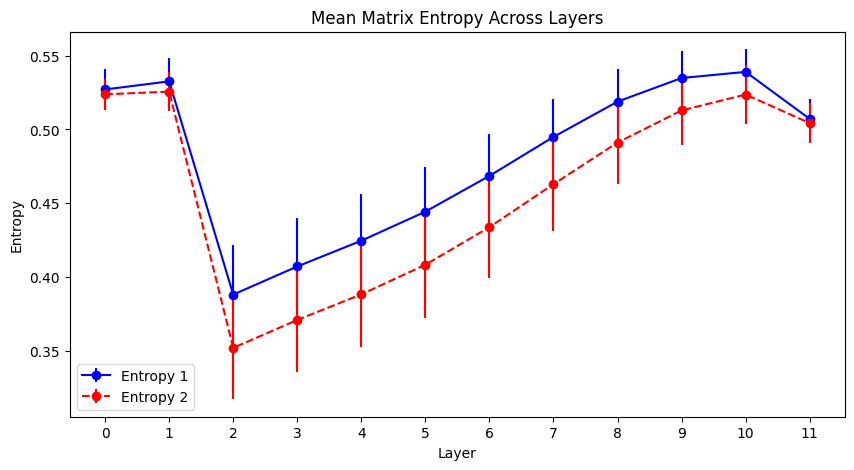
\includegraphics[width=\linewidth]{Small_World_Stories.png}
        \caption{GPT-2 Small (85M) World Stories}
        \label{fig:small_world_stories}
    \end{minipage}\hfill
    \begin{minipage}{0.5\linewidth}
        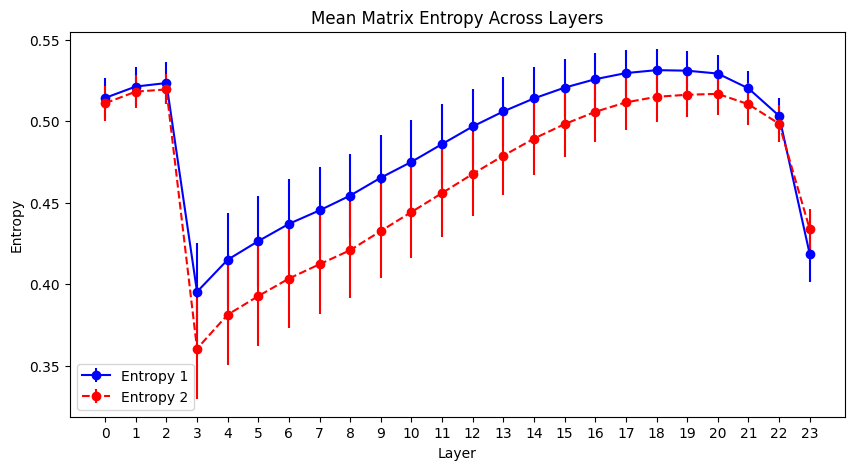
\includegraphics[width=\linewidth]{Medium_World_Stories.png}
        \caption{GPT-2 Medium (302M) World Stories}
        \label{fig:medium_world_stories}
    \end{minipage}\hfill
\end{figure}



\begin{figure} [H]
\centering
    \begin{minipage}{0.5\linewidth}
        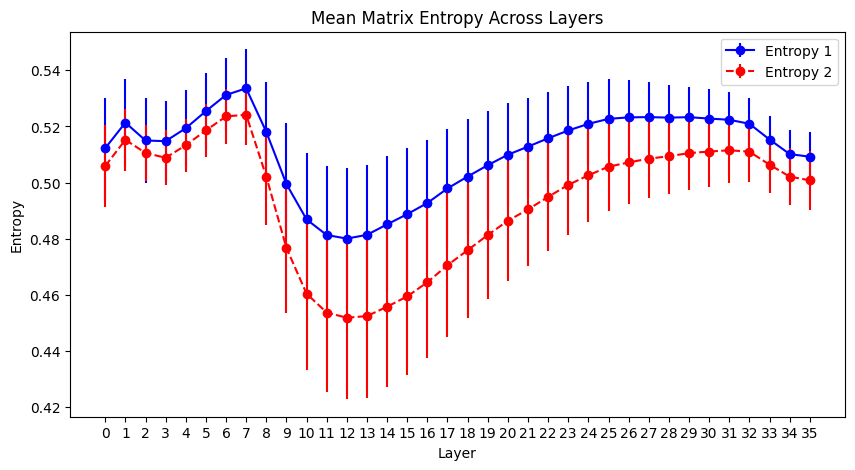
\includegraphics[width=\linewidth]{Large_World_Stories.png}
        \caption{GPT-2 Large (708M) World Stories}
        \label{fig:large_world_stories}
    \end{minipage}
\end{figure}




\section{Observation}

\subsection{Datasets}
In analyzing the matrix entropy across layers for different models with varying capacities, distinct observations emerge when processing two specific datasets: child stories and world stories. These findings shed light on the nuanced capabilities and potential limitations of these models when handling thematic content.

For child stories, which included good, bad, and their condensed versions, the models consistently exhibited higher entropy values for narratives categorized as "good" compared to their "bad" counterparts. This suggests that the models are capable of discerning and intricately processing narratives that are richer in content and structure. The larger models, specifically the Medium and Large versions, displayed more consistent entropy values across layers, indicating a stable handling of narrative complexities.

On the other hand, the world stories dataset, comprising utopian and dystopian narratives, showed more varied entropy trends. Utopian stories generally exhibited higher entropy across all models, indicating a strong and consistent processing of these idealistic themes. Dystopian stories, however, presented greater variability, particularly in the large model, reflecting a complex interaction with these often darker and more varied narratives. The significant standard deviation in entropy values across layers in the large model suggests its capacity for deep, nuanced interpretation of complex themes, though this also resulted in less predictability in processing outcomes.

\subsection{Models}

One clear observation is the models' sensitivity to narrative quality. There is a noticeable trend where well-crafted stories—whether they are good child stories or utopian world stories—tend to produce higher entropy values. This suggests that these models are adept at recognizing and processing well-structured stories with greater complexity, highlighting their capability to discern narrative quality and respond with appropriate complexity in their processing strategies.

Another important factor is the impact of model size on entropy behavior across layers. Increasing the size of the models generally results in a smoother entropy curve, which suggests an enhanced ability to handle narrative complexity consistently. However, with larger models, particularly evident in the large model processing world stories, there is an introduction of greater variability in how individual layers react to the content. This indicates a nuanced but less uniform processing capability, which may reflect deeper, more nuanced engagements with complex themes but also highlights potential challenges in maintaining processing consistency across different layers.

Furthermore, the thematic processing capabilities of these models demonstrate their diverse strengths and challenges. The handling of child stories, which are typically simpler and more linear, shows more predictability across all model sizes. This contrasts with the processing of world stories, which often carry more layered and complex themes. These narratives challenge the models in unique ways, especially the larger models, which display both the capacity for deep thematic analysis and the challenge of maintaining consistent processing across their extensive layer structures.

Overall, these insights underscore the sophisticated nature of language models in dealing with narrative complexity and thematic depth, revealing how model architecture and size can influence their ability to process and interpret diverse literary genres effectively.


\section{Conclusion}


This study has provided valuable insights into how different LLMs process narratives of varying complexities and themes, highlighting the importance of model size and narrative quality on entropy behaviors across layers. It is evident that larger models, while capable of nuanced processing, exhibit greater variability in layer responses, suggesting both an opportunity for deep thematic analysis and a challenge in maintaining consistency. The differential processing of child versus world stories further illustrates the model's adaptability to narrative structure and complexity. For future work, it would be beneficial to expand this analysis to include a broader range of datasets. Testing diverse literary genres and thematic content across models could further elucidate how changes in model architecture influence processing capabilities across layers, potentially guiding enhancements in model training and design to better handle a wider array of narrative complexities.

The results from this study also significantly contribute to the field of machine learning and model interpretability. By analyzing entropy across model layers, we gain a deeper understanding of how different neural network architectures encode and interpret information. This kind of analysis is crucial for the development of more interpretable machine learning models, as it helps delineate which parts of a model are most sensitive to certain types of input and how information flows and transforms throughout the network. Such insights are invaluable for improving model transparency and trustworthiness, crucial aspects in the deployment of AI systems in real-world applications where decisions need to be understood and justified. Future explorations involving varied datasets will not only validate these findings but also refine our approaches to building more robust and interpretable models.







\section{Acknowledgements}
Much appreciation for professor Michael Ivanitskiy for helping me use the transformer lens package, giving me advice on experimental directions and think this is a valid project idea. Also thank so much for professor Samy Wu Fung for giving me advice on experimental directions and acknowledged that this will be funny idea to work on.




\bibliographystyle{unsrt}
\bibliography{yourref.bib}





%%%%%%%%%%%%%%%%%%%%%%%%%%%%%%%%%%%%%%%%%%%%%%%%%%%%%%%%%%%%

\end{document}